The inner detector (ID) is designed to provide good track reconstruction,
precise momentum resolution and both primary and secondary vertex measurements
above a nominal $\pt$ threshold of 0.5~GeV and within the pseudorapidity
$|\eta| < 2.5$. It also provides electron identification over $|\eta| < 2.0$ for
energies between 0.5~GeV and 150~GeV\cite{ATLASPaper}. The ID is 6.2~m long and
has a radius of about 1.1~m, it is surrounded by a solenoidal magnetic field of
2~T. Its layout is schematized in Figure~\ref{fig:id} and, as can be seen, it is
composed of three sub-detectors. At the inner radius the \emph{pixel detector}
mostly determines the position of primary and secondary vertex. The silicon
sensors are 250~$\mu$m thick detectors that operate with an initial bias voltage
of $\sim$150~V that will increase up to 600~V after 10 years of operation. In
the middle layer of the ID the \emph{semiconductor tracker} (SCT) is designed to
give eight precision measurements per track which contributes to the primary and
secondary vertex position and momentum measurements. The silicon sensors are 285
$\pm 15 \mu$m thick and initially operated with a bias voltage of $\sim$150
position
\begin{figure}[!h]
  \centering
    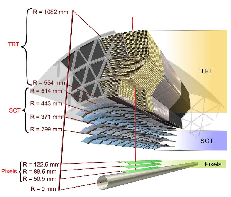
\includegraphics[width=.5\linewidth]{inner_detector}
    \caption{Schematic view of a charged track of 10~GeV $\pt$ that traverses
      the different ID sub-detectors. After traversing the beryllium pipe, the
      track passes through the three cylindrical silicon-pixel layers, the four
      layers of silicon-microstrip sensors (SCT) and the approximately 36 straws
      contained in the TRT within their support structure.}
    \label{fig:id}
\end{figure}
%%% Local Variables:
%%% mode: latex
%%% TeX-master: "../search_for_DM_LED_with_ATLAS"
%%% End:
